% Options for packages loaded elsewhere
\PassOptionsToPackage{unicode}{hyperref}
\PassOptionsToPackage{hyphens}{url}
%
\documentclass[
]{article}
\usepackage{amsmath,amssymb}
\usepackage{iftex}
\ifPDFTeX
  \usepackage[T1]{fontenc}
  \usepackage[utf8]{inputenc}
  \usepackage{textcomp} % provide euro and other symbols
\else % if luatex or xetex
  \usepackage{unicode-math} % this also loads fontspec
  \defaultfontfeatures{Scale=MatchLowercase}
  \defaultfontfeatures[\rmfamily]{Ligatures=TeX,Scale=1}
\fi
\usepackage{lmodern}
\ifPDFTeX\else
  % xetex/luatex font selection
\fi
% Use upquote if available, for straight quotes in verbatim environments
\IfFileExists{upquote.sty}{\usepackage{upquote}}{}
\IfFileExists{microtype.sty}{% use microtype if available
  \usepackage[]{microtype}
  \UseMicrotypeSet[protrusion]{basicmath} % disable protrusion for tt fonts
}{}
\makeatletter
\@ifundefined{KOMAClassName}{% if non-KOMA class
  \IfFileExists{parskip.sty}{%
    \usepackage{parskip}
  }{% else
    \setlength{\parindent}{0pt}
    \setlength{\parskip}{6pt plus 2pt minus 1pt}}
}{% if KOMA class
  \KOMAoptions{parskip=half}}
\makeatother
\usepackage{xcolor}
\usepackage[margin=1in]{geometry}
\usepackage{color}
\usepackage{fancyvrb}
\newcommand{\VerbBar}{|}
\newcommand{\VERB}{\Verb[commandchars=\\\{\}]}
\DefineVerbatimEnvironment{Highlighting}{Verbatim}{commandchars=\\\{\}}
% Add ',fontsize=\small' for more characters per line
\usepackage{framed}
\definecolor{shadecolor}{RGB}{248,248,248}
\newenvironment{Shaded}{\begin{snugshade}}{\end{snugshade}}
\newcommand{\AlertTok}[1]{\textcolor[rgb]{0.94,0.16,0.16}{#1}}
\newcommand{\AnnotationTok}[1]{\textcolor[rgb]{0.56,0.35,0.01}{\textbf{\textit{#1}}}}
\newcommand{\AttributeTok}[1]{\textcolor[rgb]{0.13,0.29,0.53}{#1}}
\newcommand{\BaseNTok}[1]{\textcolor[rgb]{0.00,0.00,0.81}{#1}}
\newcommand{\BuiltInTok}[1]{#1}
\newcommand{\CharTok}[1]{\textcolor[rgb]{0.31,0.60,0.02}{#1}}
\newcommand{\CommentTok}[1]{\textcolor[rgb]{0.56,0.35,0.01}{\textit{#1}}}
\newcommand{\CommentVarTok}[1]{\textcolor[rgb]{0.56,0.35,0.01}{\textbf{\textit{#1}}}}
\newcommand{\ConstantTok}[1]{\textcolor[rgb]{0.56,0.35,0.01}{#1}}
\newcommand{\ControlFlowTok}[1]{\textcolor[rgb]{0.13,0.29,0.53}{\textbf{#1}}}
\newcommand{\DataTypeTok}[1]{\textcolor[rgb]{0.13,0.29,0.53}{#1}}
\newcommand{\DecValTok}[1]{\textcolor[rgb]{0.00,0.00,0.81}{#1}}
\newcommand{\DocumentationTok}[1]{\textcolor[rgb]{0.56,0.35,0.01}{\textbf{\textit{#1}}}}
\newcommand{\ErrorTok}[1]{\textcolor[rgb]{0.64,0.00,0.00}{\textbf{#1}}}
\newcommand{\ExtensionTok}[1]{#1}
\newcommand{\FloatTok}[1]{\textcolor[rgb]{0.00,0.00,0.81}{#1}}
\newcommand{\FunctionTok}[1]{\textcolor[rgb]{0.13,0.29,0.53}{\textbf{#1}}}
\newcommand{\ImportTok}[1]{#1}
\newcommand{\InformationTok}[1]{\textcolor[rgb]{0.56,0.35,0.01}{\textbf{\textit{#1}}}}
\newcommand{\KeywordTok}[1]{\textcolor[rgb]{0.13,0.29,0.53}{\textbf{#1}}}
\newcommand{\NormalTok}[1]{#1}
\newcommand{\OperatorTok}[1]{\textcolor[rgb]{0.81,0.36,0.00}{\textbf{#1}}}
\newcommand{\OtherTok}[1]{\textcolor[rgb]{0.56,0.35,0.01}{#1}}
\newcommand{\PreprocessorTok}[1]{\textcolor[rgb]{0.56,0.35,0.01}{\textit{#1}}}
\newcommand{\RegionMarkerTok}[1]{#1}
\newcommand{\SpecialCharTok}[1]{\textcolor[rgb]{0.81,0.36,0.00}{\textbf{#1}}}
\newcommand{\SpecialStringTok}[1]{\textcolor[rgb]{0.31,0.60,0.02}{#1}}
\newcommand{\StringTok}[1]{\textcolor[rgb]{0.31,0.60,0.02}{#1}}
\newcommand{\VariableTok}[1]{\textcolor[rgb]{0.00,0.00,0.00}{#1}}
\newcommand{\VerbatimStringTok}[1]{\textcolor[rgb]{0.31,0.60,0.02}{#1}}
\newcommand{\WarningTok}[1]{\textcolor[rgb]{0.56,0.35,0.01}{\textbf{\textit{#1}}}}
\usepackage{graphicx}
\makeatletter
\def\maxwidth{\ifdim\Gin@nat@width>\linewidth\linewidth\else\Gin@nat@width\fi}
\def\maxheight{\ifdim\Gin@nat@height>\textheight\textheight\else\Gin@nat@height\fi}
\makeatother
% Scale images if necessary, so that they will not overflow the page
% margins by default, and it is still possible to overwrite the defaults
% using explicit options in \includegraphics[width, height, ...]{}
\setkeys{Gin}{width=\maxwidth,height=\maxheight,keepaspectratio}
% Set default figure placement to htbp
\makeatletter
\def\fps@figure{htbp}
\makeatother
\setlength{\emergencystretch}{3em} % prevent overfull lines
\providecommand{\tightlist}{%
  \setlength{\itemsep}{0pt}\setlength{\parskip}{0pt}}
\setcounter{secnumdepth}{-\maxdimen} % remove section numbering
\usepackage{fvextra}
\DefineVerbatimEnvironment{Highlighting}{Verbatim}{breaklines,commandchars=\\\{\}}
\ifLuaTeX
  \usepackage{selnolig}  % disable illegal ligatures
\fi
\usepackage{bookmark}
\IfFileExists{xurl.sty}{\usepackage{xurl}}{} % add URL line breaks if available
\urlstyle{same}
\hypersetup{
  pdftitle={SDA Group Submission Assignment Assign1},
  pdfauthor={MengliFeng (2720589) and PepijnVanOostveen (2801582)},
  hidelinks,
  pdfcreator={LaTeX via pandoc}}

\title{SDA Group Submission Assignment Assign1}
\usepackage{etoolbox}
\makeatletter
\providecommand{\subtitle}[1]{% add subtitle to \maketitle
  \apptocmd{\@title}{\par {\large #1 \par}}{}{}
}
\makeatother
\subtitle{Group Gr18}
\author{MengliFeng (2720589) and PepijnVanOostveen (2801582)}
\date{}

\begin{document}
\maketitle

\section{Exercise 1}\label{exercise-1}

\subsection{a.}\label{a.}

\begin{Shaded}
\begin{Highlighting}[]
\NormalTok{CTL\_unif }\OtherTok{\textless{}{-}} \ControlFlowTok{function}\NormalTok{(n,m)\{}
  \CommentTok{\# Use replicate to generate n samples, each consisting of m draws from U(0, 1)}
\NormalTok{  sample\_means }\OtherTok{\textless{}{-}} \FunctionTok{replicate}\NormalTok{(n, }\FunctionTok{mean}\NormalTok{(}\FunctionTok{runif}\NormalTok{(m)))}
  
  \CommentTok{\# Return the vector of sample means}
  \FunctionTok{return}\NormalTok{(sample\_means)}
\NormalTok{\}}
\end{Highlighting}
\end{Shaded}

\subsection{b.}\label{b.}

\begin{Shaded}
\begin{Highlighting}[]
\CommentTok{\# Set seed for reproducibility}
\FunctionTok{set.seed}\NormalTok{(}\DecValTok{42}\NormalTok{)}

\CommentTok{\# Generate sample means for n = 500, m = 30}
\NormalTok{means\_30 }\OtherTok{\textless{}{-}} \FunctionTok{CTL\_unif}\NormalTok{(}\AttributeTok{n =} \DecValTok{500}\NormalTok{, }\AttributeTok{m =} \DecValTok{30}\NormalTok{)}

\CommentTok{\# Generate sample means for n = 500, m = 200}
\NormalTok{means\_200 }\OtherTok{\textless{}{-}} \FunctionTok{CTL\_unif}\NormalTok{(}\AttributeTok{n =} \DecValTok{500}\NormalTok{, }\AttributeTok{m =} \DecValTok{200}\NormalTok{)}

\CommentTok{\# Define the parameters for the normal distribution}
\NormalTok{mean\_theoretical }\OtherTok{\textless{}{-}} \FloatTok{0.5}
\NormalTok{sd\_30 }\OtherTok{\textless{}{-}} \FunctionTok{sqrt}\NormalTok{(}\DecValTok{1} \SpecialCharTok{/}\NormalTok{ (}\DecValTok{12} \SpecialCharTok{*} \DecValTok{30}\NormalTok{))  }\CommentTok{\# Standard deviation for m = 30}
\NormalTok{sd\_200 }\OtherTok{\textless{}{-}} \FunctionTok{sqrt}\NormalTok{(}\DecValTok{1} \SpecialCharTok{/}\NormalTok{ (}\DecValTok{12} \SpecialCharTok{*} \DecValTok{200}\NormalTok{))  }\CommentTok{\# Standard deviation for m = 200}

\CommentTok{\# Get dynamic ylim values based on the density range}
\NormalTok{ylim\_30 }\OtherTok{\textless{}{-}} \FunctionTok{c}\NormalTok{(}\DecValTok{0}\NormalTok{, }\FunctionTok{max}\NormalTok{(}\FunctionTok{density}\NormalTok{(means\_30)}\SpecialCharTok{$}\NormalTok{y, }\FunctionTok{dnorm}\NormalTok{(mean\_theoretical, }\AttributeTok{mean =}\NormalTok{ mean\_theoretical, }\AttributeTok{sd =}\NormalTok{ sd\_30)))}
\NormalTok{ylim\_200 }\OtherTok{\textless{}{-}} \FunctionTok{c}\NormalTok{(}\DecValTok{0}\NormalTok{, }\FunctionTok{max}\NormalTok{(}\FunctionTok{density}\NormalTok{(means\_200)}\SpecialCharTok{$}\NormalTok{y, }\FunctionTok{dnorm}\NormalTok{(mean\_theoretical, }\AttributeTok{mean =}\NormalTok{ mean\_theoretical, }\AttributeTok{sd =}\NormalTok{ sd\_200)))}

\CommentTok{\# Plot the histograms side{-}by{-}side}
\FunctionTok{par}\NormalTok{(}\AttributeTok{mfrow =} \FunctionTok{c}\NormalTok{(}\DecValTok{1}\NormalTok{, }\DecValTok{2}\NormalTok{))  }\CommentTok{\# Set up a 1x2 plotting layout}

\CommentTok{\# Plot for m = 30}
\FunctionTok{hist}\NormalTok{(means\_30, }\AttributeTok{prob =} \ConstantTok{TRUE}\NormalTok{, }\AttributeTok{xlim =} \FunctionTok{c}\NormalTok{(}\FloatTok{0.3}\NormalTok{, }\FloatTok{0.7}\NormalTok{), }\AttributeTok{ylim =}\NormalTok{ ylim\_30,}
     \AttributeTok{main =} \StringTok{"Histogram for m = 30"}\NormalTok{, }\AttributeTok{xlab =} \StringTok{"Sample Mean"}\NormalTok{)}
\FunctionTok{curve}\NormalTok{(}\FunctionTok{dnorm}\NormalTok{(x, }\AttributeTok{mean =}\NormalTok{ mean\_theoretical, }\AttributeTok{sd =}\NormalTok{ sd\_30), }\AttributeTok{col =} \StringTok{"blue"}\NormalTok{, }\AttributeTok{lwd =} \DecValTok{2}\NormalTok{, }\AttributeTok{add =} \ConstantTok{TRUE}\NormalTok{)}

\CommentTok{\# Plot for m = 200}
\FunctionTok{hist}\NormalTok{(means\_200, }\AttributeTok{prob =} \ConstantTok{TRUE}\NormalTok{, }\AttributeTok{xlim =} \FunctionTok{c}\NormalTok{(}\FloatTok{0.3}\NormalTok{, }\FloatTok{0.7}\NormalTok{), }\AttributeTok{ylim =}\NormalTok{ ylim\_200,}
     \AttributeTok{main =} \StringTok{"Histogram for m = 200"}\NormalTok{, }\AttributeTok{xlab =} \StringTok{"Sample Mean"}\NormalTok{)}
\FunctionTok{curve}\NormalTok{(}\FunctionTok{dnorm}\NormalTok{(x, }\AttributeTok{mean =}\NormalTok{ mean\_theoretical, }\AttributeTok{sd =}\NormalTok{ sd\_200), }\AttributeTok{col =} \StringTok{"red"}\NormalTok{, }\AttributeTok{lwd =} \DecValTok{2}\NormalTok{, }\AttributeTok{add =} \ConstantTok{TRUE}\NormalTok{)}
\end{Highlighting}
\end{Shaded}

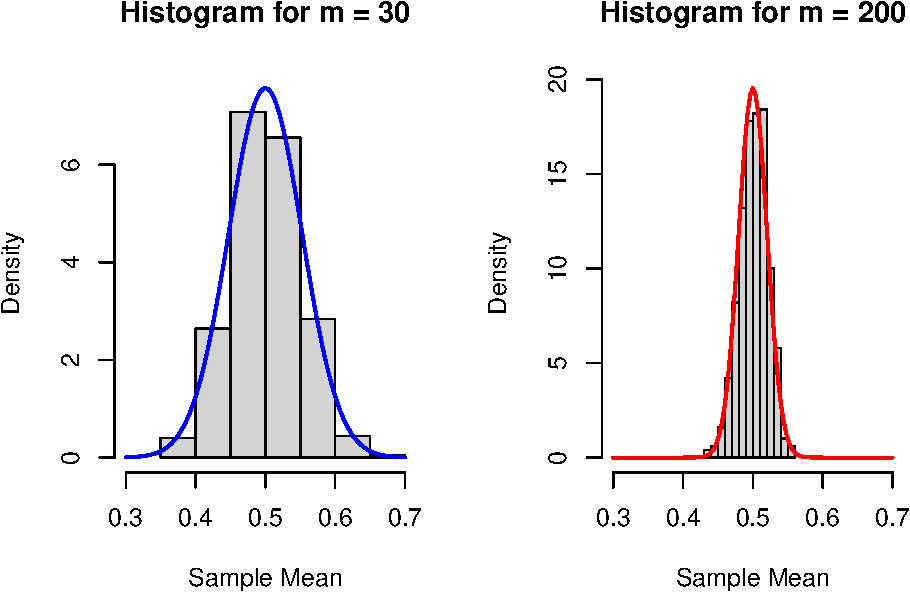
\includegraphics{SDA_submission_template_files/figure-latex/unnamed-chunk-2-1.pdf}

\begin{Shaded}
\begin{Highlighting}[]
\CommentTok{\# Reset the plotting layout}
\FunctionTok{par}\NormalTok{(}\AttributeTok{mfrow =} \FunctionTok{c}\NormalTok{(}\DecValTok{1}\NormalTok{, }\DecValTok{1}\NormalTok{))}
\end{Highlighting}
\end{Shaded}

\subsection{c.}\label{c.}

we can observe that when we take more samples in each draw, the variance
of the distribution of the sample means is smaller. And overall, we can
see the distribution of the sample means converges to the theoretical
distribution as the sample size in each draw increases. This can be
explained by central limit theorem.

\section{Exercise 2}\label{exercise-2}

\begin{Shaded}
\begin{Highlighting}[]
\FunctionTok{data}\NormalTok{(}\StringTok{"airquality"}\NormalTok{)}
\FunctionTok{head}\NormalTok{(airquality)}
\end{Highlighting}
\end{Shaded}

\begin{verbatim}
##   Ozone Solar.R Wind Temp Month Day
## 1    41     190  7.4   67     5   1
## 2    36     118  8.0   72     5   2
## 3    12     149 12.6   74     5   3
## 4    18     313 11.5   62     5   4
## 5    NA      NA 14.3   56     5   5
## 6    28      NA 14.9   66     5   6
\end{verbatim}

\subsection{a.}\label{a.-1}

\begin{Shaded}
\begin{Highlighting}[]
\CommentTok{\# It isn\textquotesingle{}t a good idea to use \textquotesingle{}airquality$Ozone == NA\textquotesingle{} since NA represents a missing value and comparing with NA always gives NA. Thus we use .is.na()}
\NormalTok{NA\_count }\OtherTok{\textless{}{-}} \FunctionTok{sum}\NormalTok{(}\FunctionTok{is.na}\NormalTok{(airquality}\SpecialCharTok{$}\NormalTok{Ozone))}

\CommentTok{\# calculate the proportion of missing values}
\NormalTok{NA\_proportion }\OtherTok{\textless{}{-}}\NormalTok{ NA\_count }\SpecialCharTok{/} \FunctionTok{nrow}\NormalTok{(airquality)}
\NormalTok{NA\_proportion}
\end{Highlighting}
\end{Shaded}

\begin{verbatim}
## [1] 0.2418301
\end{verbatim}

\begin{Shaded}
\begin{Highlighting}[]
\CommentTok{\# na.rm = TRUE ensures a numerical output since it removes the missing values as it stands for na.remove}
\NormalTok{mean\_ozone }\OtherTok{\textless{}{-}} \FunctionTok{mean}\NormalTok{(airquality}\SpecialCharTok{$}\NormalTok{Ozone, }\AttributeTok{na.rm =} \ConstantTok{TRUE}\NormalTok{)}
\NormalTok{mean\_ozone}
\end{Highlighting}
\end{Shaded}

\begin{verbatim}
## [1] 42.12931
\end{verbatim}

\subsection{b.}\label{b.-1}

\begin{Shaded}
\begin{Highlighting}[]
\CommentTok{\# remove all rows with a missing value}
\NormalTok{airquality\_clean }\OtherTok{\textless{}{-}} \FunctionTok{na.omit}\NormalTok{(airquality)}

\CommentTok{\# remove the Day and Month columns}
\NormalTok{airquality\_clean }\OtherTok{\textless{}{-}} \FunctionTok{subset}\NormalTok{(airquality\_clean, }\AttributeTok{select =} \SpecialCharTok{{-}}\FunctionTok{c}\NormalTok{(Month, Day))}

\CommentTok{\# make a summarry for every column}
\FunctionTok{summary}\NormalTok{(airquality\_clean)}
\end{Highlighting}
\end{Shaded}

\begin{verbatim}
##      Ozone          Solar.R           Wind            Temp      
##  Min.   :  1.0   Min.   :  7.0   Min.   : 2.30   Min.   :57.00  
##  1st Qu.: 18.0   1st Qu.:113.5   1st Qu.: 7.40   1st Qu.:71.00  
##  Median : 31.0   Median :207.0   Median : 9.70   Median :79.00  
##  Mean   : 42.1   Mean   :184.8   Mean   : 9.94   Mean   :77.79  
##  3rd Qu.: 62.0   3rd Qu.:255.5   3rd Qu.:11.50   3rd Qu.:84.50  
##  Max.   :168.0   Max.   :334.0   Max.   :20.70   Max.   :97.00
\end{verbatim}

\begin{Shaded}
\begin{Highlighting}[]
\CommentTok{\# make the layout of boxplots a 2x2 grid}
\FunctionTok{par}\NormalTok{(}\AttributeTok{mfrow =} \FunctionTok{c}\NormalTok{(}\DecValTok{2}\NormalTok{, }\DecValTok{2}\NormalTok{))}

\CommentTok{\# one by one plot all 4 of the boxplots}
\FunctionTok{boxplot}\NormalTok{(airquality\_clean}\SpecialCharTok{$}\NormalTok{Ozone, }\AttributeTok{main =} \StringTok{"Ozone"}\NormalTok{)}
\FunctionTok{boxplot}\NormalTok{(airquality\_clean}\SpecialCharTok{$}\NormalTok{Solar.R, }\AttributeTok{main =} \StringTok{"Solar Radiation"}\NormalTok{)}
\FunctionTok{boxplot}\NormalTok{(airquality\_clean}\SpecialCharTok{$}\NormalTok{Wind, }\AttributeTok{main =} \StringTok{"Wind"}\NormalTok{)}
\FunctionTok{boxplot}\NormalTok{(airquality\_clean}\SpecialCharTok{$}\NormalTok{Temp, }\AttributeTok{main =} \StringTok{"Temperature"}\NormalTok{)}
\end{Highlighting}
\end{Shaded}

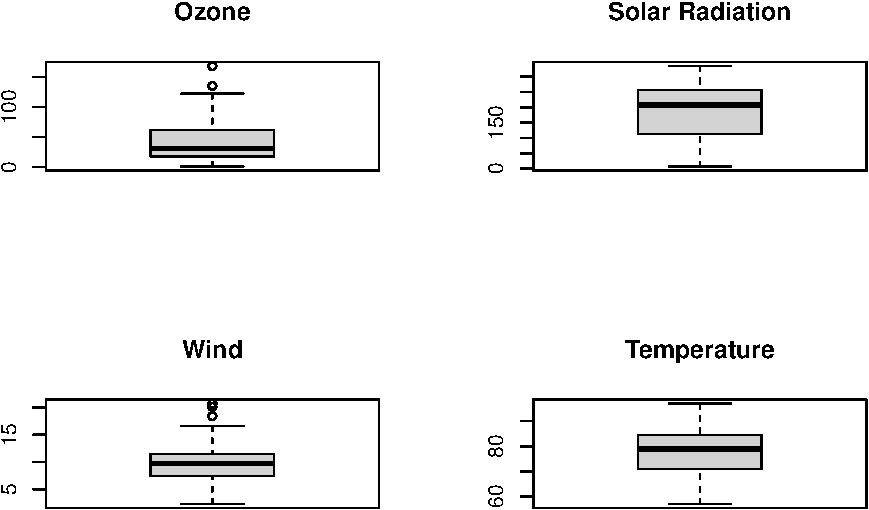
\includegraphics{SDA_submission_template_files/figure-latex/unnamed-chunk-5-1.pdf}

\begin{Shaded}
\begin{Highlighting}[]
\CommentTok{\# reset layout}
\FunctionTok{par}\NormalTok{(}\AttributeTok{mfrow =} \FunctionTok{c}\NormalTok{(}\DecValTok{1}\NormalTok{, }\DecValTok{1}\NormalTok{))}
\end{Highlighting}
\end{Shaded}

\subsection{c.}\label{c.-1}

\begin{Shaded}
\begin{Highlighting}[]
\CommentTok{\# correlation between Ozone and Temp}
\FunctionTok{cor}\NormalTok{(airquality\_clean}\SpecialCharTok{$}\NormalTok{Ozone, airquality\_clean}\SpecialCharTok{$}\NormalTok{Temp)}
\end{Highlighting}
\end{Shaded}

\begin{verbatim}
## [1] 0.6985414
\end{verbatim}

\begin{Shaded}
\begin{Highlighting}[]
\CommentTok{\# correlation between square root of Ozone and Temp}
\FunctionTok{cor}\NormalTok{(}\FunctionTok{sqrt}\NormalTok{(airquality\_clean}\SpecialCharTok{$}\NormalTok{Ozone), airquality\_clean}\SpecialCharTok{$}\NormalTok{Temp)}
\end{Highlighting}
\end{Shaded}

\begin{verbatim}
## [1] 0.7458552
\end{verbatim}

\begin{Shaded}
\begin{Highlighting}[]
\CommentTok{\# The correlation changes between these two and it is higher for sqrt Ozone vs Temp, thus that has a better correlation}

\CommentTok{\# use a 1x2 grid so the plots are beside each other}
\FunctionTok{par}\NormalTok{(}\AttributeTok{mfrow =} \FunctionTok{c}\NormalTok{(}\DecValTok{1}\NormalTok{, }\DecValTok{2}\NormalTok{))}

\CommentTok{\# plot Ozone vs Temp}
\FunctionTok{plot}\NormalTok{(airquality\_clean}\SpecialCharTok{$}\NormalTok{Ozone, airquality\_clean}\SpecialCharTok{$}\NormalTok{Temp, }
     \AttributeTok{main =} \StringTok{"Ozone vs Temp"}\NormalTok{, }\AttributeTok{xlab =} \StringTok{"Ozone"}\NormalTok{, }\AttributeTok{ylab =} \StringTok{"Temperature"}\NormalTok{)}

\CommentTok{\# plot sqrt Ozone vs Temp}
\FunctionTok{plot}\NormalTok{(}\FunctionTok{sqrt}\NormalTok{(airquality\_clean}\SpecialCharTok{$}\NormalTok{Ozone), airquality\_clean}\SpecialCharTok{$}\NormalTok{Temp, }
     \AttributeTok{main =} \StringTok{"sqrt Ozone vs Temp"}\NormalTok{, }\AttributeTok{xlab =} \StringTok{"sqrt Ozone"}\NormalTok{, }\AttributeTok{ylab =} \StringTok{"Temperature"}\NormalTok{)}
\end{Highlighting}
\end{Shaded}

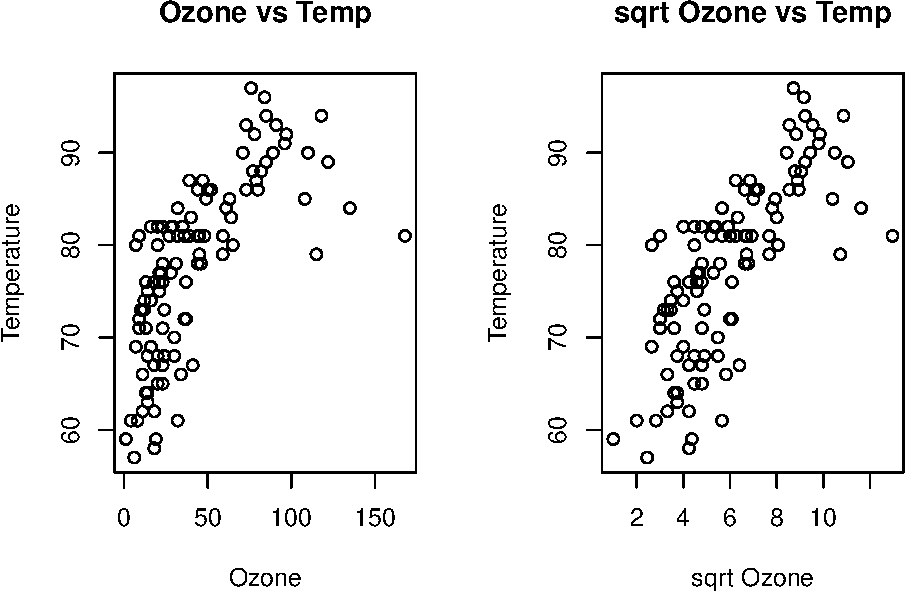
\includegraphics{SDA_submission_template_files/figure-latex/unnamed-chunk-6-1.pdf}

\begin{Shaded}
\begin{Highlighting}[]
\CommentTok{\# Both have a lot of variation but the second plot follows a line better so that one more closely resembles a linear relationship}
\end{Highlighting}
\end{Shaded}


\end{document}
